\section{Drosophila brain regions}

\begin{enumerate}
    \item \tb{OL}: \href{https://en.wikipedia.org/wiki/Optic_lobe_(arthropods)}{Optical lobe}. sits behind the arthropod eye (mostly compound eyes) 
        and is responsible for the processing of the visual information. It is made up of three layers:
        \begin{enumerate}
            \item Lamina (ganglionaris): responsible for contrast enhancement through lateral inhibition
            \item Medulla: processes movement and shows movement direction sensitivity. Possesses local motion detectors
            \item Lobula: integrates information from large areas of the visual field to abstract visual information and object recognition
        \end{enumerate}
    \item \tb{MB}: \href{https://en.wikipedia.org/wiki/Mushroom_bodies}{Mushroom body}. They are also known to play a role in olfactory learning and memory. In most insects, 
        the mushroom bodies and the lateral horn are the two higher brain regions that receive olfactory information from the antennal lobe via projection neurons
    \item \tb{CX}: \href{https://www.sdbonline.org/sites/fly/aimorph/centralcomplex.htm}{Central complex}, navigation, sleep, learning, memory, nociception
    \item \tb{LX}: Lateral complex, I think that has the same function of the central complex but it is 
        lateral.
    \item \tb{VLNP}: Ventrolateral neuropils
    \item \tb{LH}: \href{https://en.wikipedia.org/wiki/Lateral_horn_of_insect_brain}{Lateral horn}.  
        It is one of the two areas of the insect brain where projection neurons of the antennal lobe send their axons. The other area is the mushroom body.
         Several morphological classes of neurons in the lateral horn receive olfactory information through the projection neurons.n lateral horn, axons of 
         pheromone-sensitive projection neurons are segregated from the axons of plant odor-sensitive projection neurons. In addition, the dendrites of lateral 
         horn neurons are restricted to one of these two zones, suggesting that pheromones and plant odors are processed separately in the lateral horn.
    \item \tb{SNP}: Superior neuropils
    \item \tb{INP}: Inferior neuropils
    \item \tb{AL}: \href{https://en.wikipedia.org/wiki/Antennal_lobe}{antennal lobe}.
    The antennal lobe is the primary (first order) olfactory brain area in insects. 
    The antennal lobe is a sphere-shaped deutocerebral neuropil in the brain that receives input
     from the olfactory sensory neurons in the antennae and mouthparts
    \item \tb{VMNP}: ventromedial neuropils
    \item \tb{PENP}: periesophageal neuropils
    \item \tb{GNG}: \href{https://www.sdbonline.org/sites/fly/aimorph/subesophagealganglion.htm}{gnathal ganglia}, taste and feeding;
\end{enumerate}

There is no clear definition for the neuropils regions, and so we provide
a definition for what the neuropils are. Neuropil (or "neuropile") is any area 
in the nervous system composed of mostly unmyelinated axons, dendrites and glial 
cell processes that forms a synaptically dense region containing a relatively low 
number of cell bodies. We can so think of them as an information bottleneck, the bridges
that connects other brain regions.
We present in Figure \ref{fig:high_lvl} a quick and not exact representation of the network between these high level
regions.
\begin{figure}[h]
    \centering
    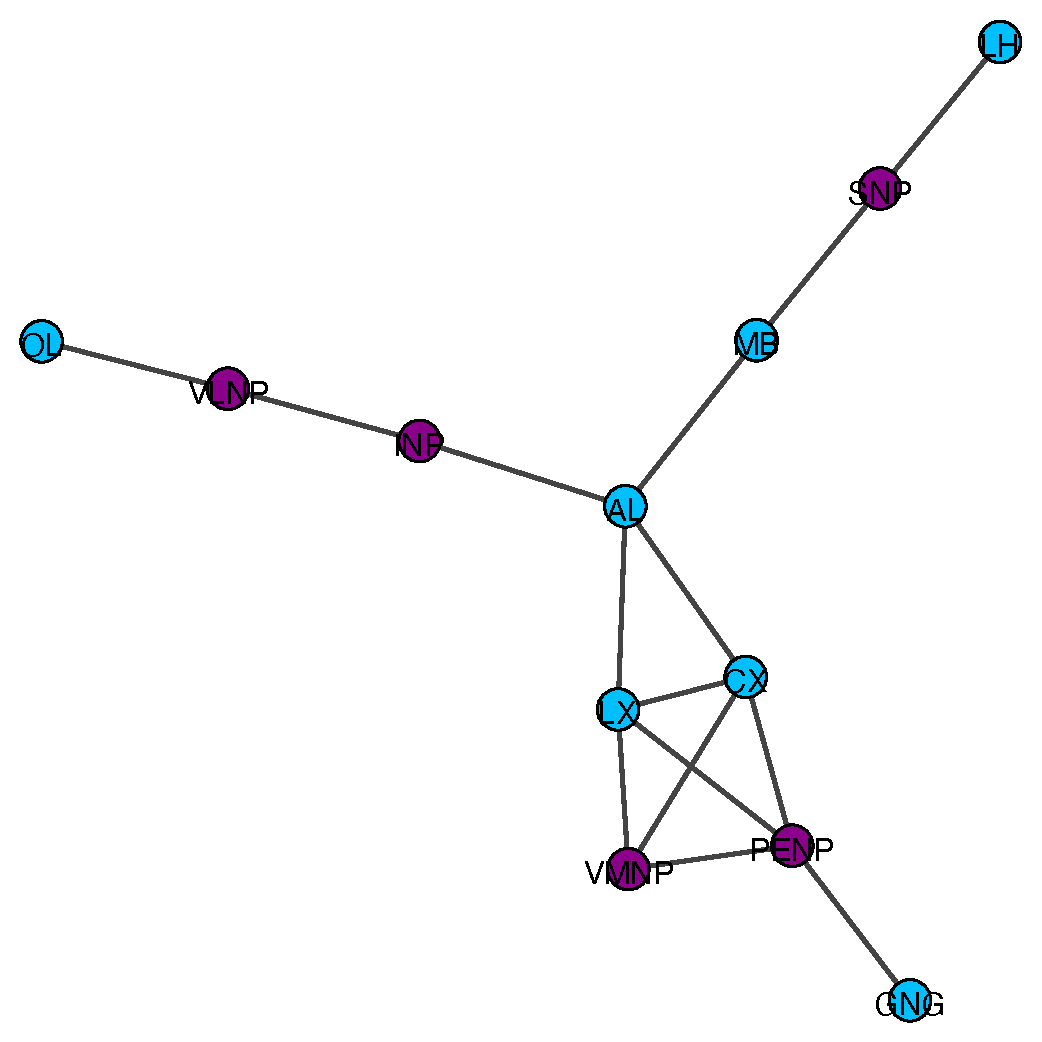
\includegraphics[width=\textwidth]{Images/high_lvl_brain.pdf}
    \caption{Approximate graph of the high level brain regions. We reported
    in magenta the neuropils. We can see even in this sketch that they act as bridges 
    between brain regions. Using another layout (tree network) we can see that the central
    complex is the central one.}
    \label{fig:high_lvl}
\end{figure}